\chapter{Architecture}
\label{chap-dev}
\label{chap-description-src}

\renewcommand{\headrulewidth}{0.3pt}
\fancyhead[LE]{\thepage} \fancyhead[RE]{\nouppercase{\textbf{\leftmark}}}
\fancyhead[RO]{\thepage} \fancyhead[LO]{\nouppercase{\textbf{\rightmark}}}
\fancyfoot[L,C,R]{}

\setlength{\parindent}{0.35cm}

\minitoc
\newpage
% ================================================================

This chapter describes the conceptual architecture --- the HTAS/CWV split and the three backend layers --- together with the \textbf{rules} a developer must follow when working within that structure, and the two entry gates through which all frontend~$\rightarrow$~backend calls must pass. The concrete recipes for extending the application and the supporting tooling follow in the next chapters.

\section{Split Architecture: HTAS and CWV}
\label{sec-split}

\cwv~is built on top of a standalone scientific backend and consumes it through a well-defined public interface. Understanding the code therefore means understanding two things: how the QGIS application and the backend are kept \emph{separate}, and how the backend is internally organised into \emph{three layers}. This section describes both, and states the strict rules a developer must follow when working within this structure.

\cwv~is maintained as two packages that are kept \textbf{strictly independent}:

\begin{itemize}
    \item \textbf{\script{HydrologicalTwinAlphaSeries} (HTAS)} --- the standalone scientific backend: simulation processing, domain structures (compartments, meshes, observations), configuration models, and the \script{HydrologicalTwin} facade. It lives under \script{external/HydrologicalTwinAlphaSeries}; in the published setup this path is a \gitlab~submodule pointing to the standalone backend repository.
    \item \textbf{\script{cawaqsviz} (CWV)} --- the standalone QGIS application: dialog boxes, visualisation workflows, GIS integration, and application-side adapters.
\end{itemize}

Independence is a hard architectural \textbf{invariant}, not a style preference:

\begin{itemize}
    \item HTAS must \textbf{never} import \script{qgis.*}, \script{PyQt5}, \script{processing}, or anything from \script{cawaqsviz/}. If you are about to add such an import inside \script{external/HydrologicalTwinAlphaSeries/}, stop --- the work belongs on the CWV side;
    \item \cwv~must consume HTAS only through its public API --- the two entry gates (\cref{sec-dev-gates}) --- and keep QGIS-specific adaptation code on the application side. Runtime HTAS imports belong in \script{interface/}; \script{frontend/} modules access backend behaviour only through the application gateway;
    \item the backend is designed to be \textbf{usable from a notebook today and a server tomorrow} (\cref{sec-notebook-usage}). Anything that breaks notebook-from-pure-Python usage also breaks the future server;
    \item synchronisation between the two repositories happens through version control and dependency pinning, not through code duplication.
\end{itemize}

\begin{figure}[htbp]
    \centering
    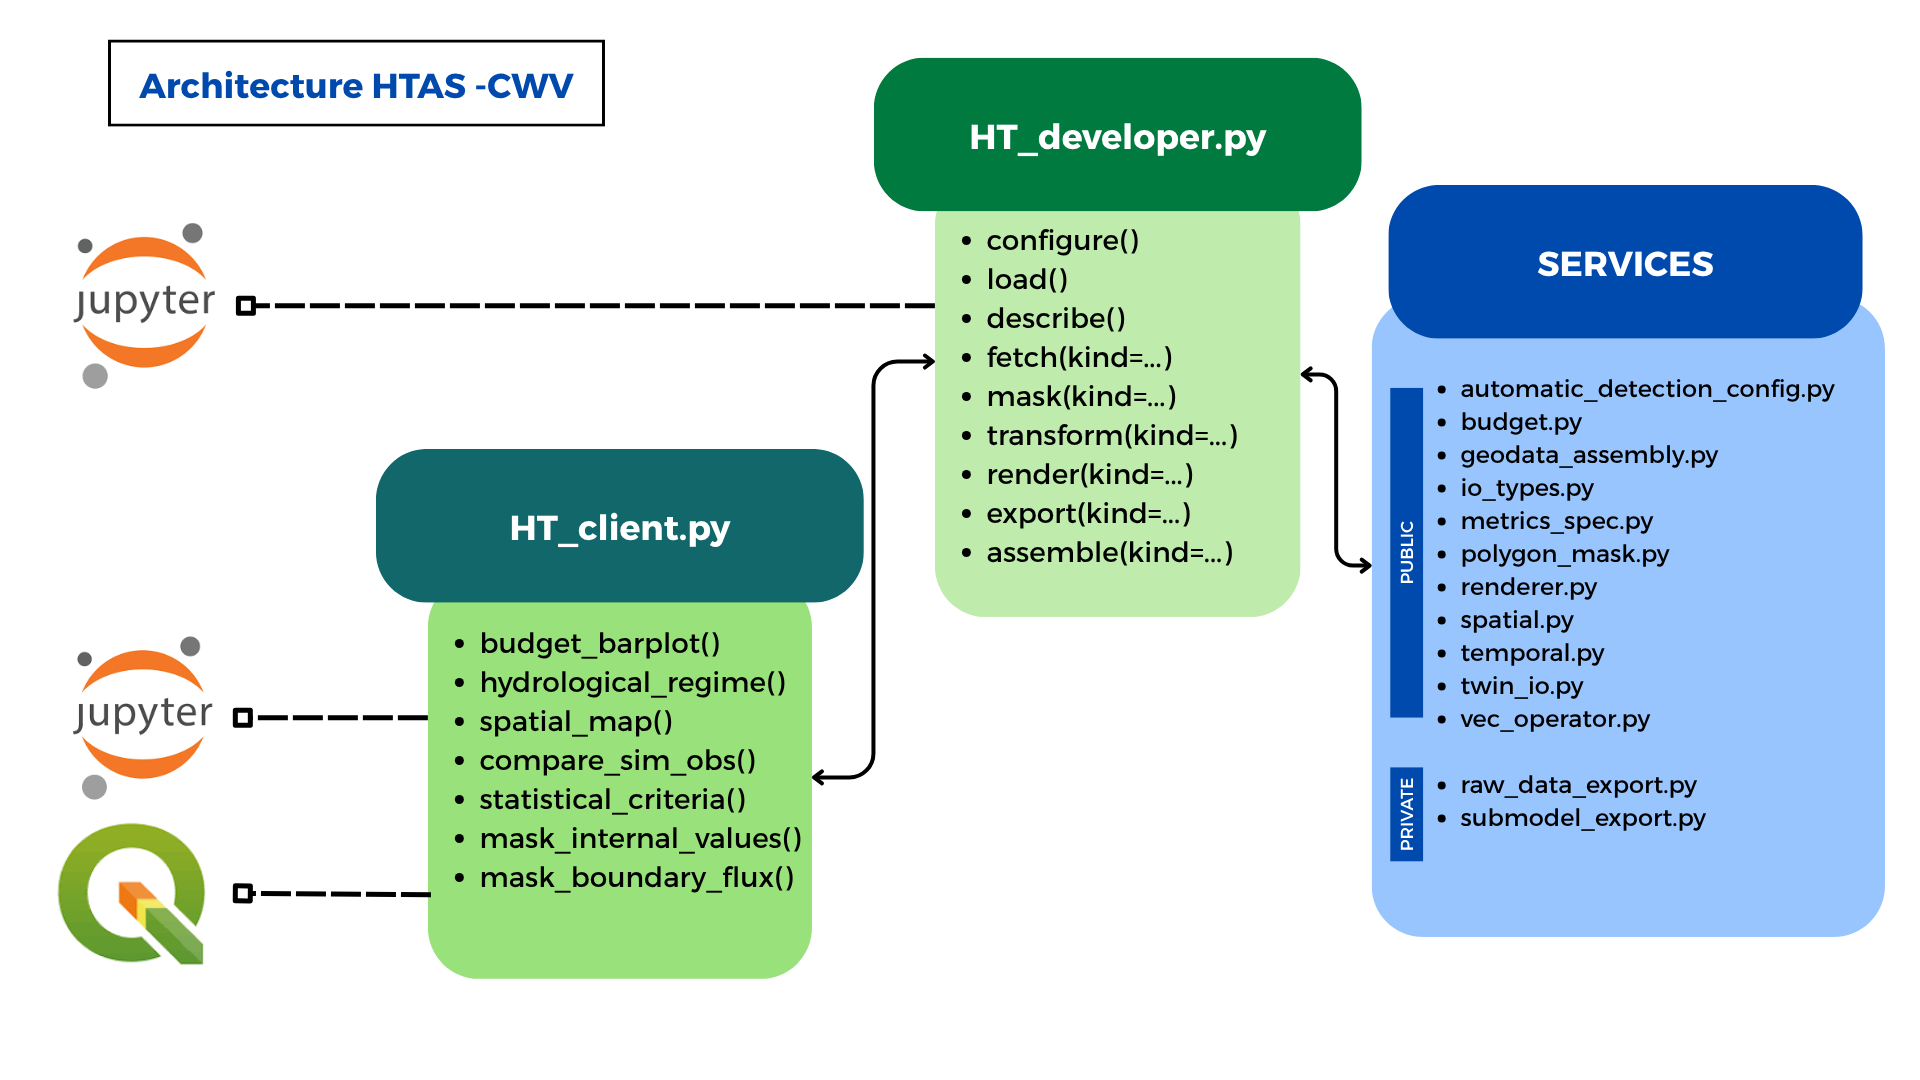
\includegraphics[width=\linewidth,height=0.85\textheight,keepaspectratio]{7_architecture/fig/architecture_developer_overview.png}
    \caption{\cwv~+~HTAS architecture. The three backend layers are L1 (\script{HT\_Client}), L2 (\script{HT\_developer}), and L3 (\script{Services}).}
    \label{fig-architecture-overview}
\end{figure}

\section{The Three Layers of the Backend}
\label{sec-layers}

HTAS is organised as a \textbf{three-level architecture} in which each level may call the level below it, never the level above. Each level has one canonical entry module, and imports point \textbf{strictly downward} (L1~$\rightarrow$~L2~$\rightarrow$~L3): never up, never sideways within a level. Because every dependency points downward, the layers can never form an import loop --- the dependency graph is acyclic.

\begin{lstlisting}[language=bash, caption={The three backend layers and their canonical entry modules.}, label={code-layers}]
L1 - HT CLIENT - MACRO        ht/client/hydrological_twin_client.py       (may import L2, L3)
L2 - HT DEVELOPER - MICRO     ht/developer/hydrological_twin_developer.py (may import L3)
L3 - SERVICES - ELEMENTARIES  services/                                   (imports nothing in ht/)
\end{lstlisting}

Taken together with the QGIS-side layers (frontend and interface), the roles are summarised in \cref{tab-layers}.

\renewcommand{\arraystretch}{1.3}
\begin{table}[H]
    \centering
    \begin{tabularx}{\linewidth}{>{\raggedright\arraybackslash}m{3.6cm}|X}
        \hline
        \textbf{Layer} & \textbf{Role} \\
        \hline
        \textbf{Frontend} \newline \script{frontend/} & QGIS dialog boxes. They own user interaction and route a single coarse call per workflow to the interface. \script{Qt}/\script{PyQt5} lives here and only here. \\
        \hline
        \textbf{Interface} \newline \script{interface/} & \script{ExploreData} is the \textbf{only} gateway to the backend; \script{GeoDataProvider} turns QGIS vector layers into \script{GeoDataFrame}s so the backend stays QGIS-agnostic. \\
        \hline
        \textbf{L1 - HT CLIENT - MACRO} \newline \script{ht/client/} & \script{HydrologicalTwinClient} exposes one method per user-facing dialog operation. Each delegates to a matching \script{operations\_client.run\_*} that owns the full \script{fetch}~$\rightarrow$~\script{transform}~$\rightarrow$~\script{render} chain and returns a typed \script{*Result} dataclass. Zero \script{qgis}/\script{PyQt5} imports --- usable from a notebook today, from an HTTP server tomorrow. \\
        \hline
        \textbf{L2 - HT DEVELOPER - MICRO} \newline \script{ht/developer/} & \script{HydrologicalTwin} is the micro-verb facade exposing 8 canonical verbs with an explicit \script{EMPTY}~$\rightarrow$~\script{CONFIGURED}~$\rightarrow$~\script{LOADED}~$\rightarrow$~\script{READY} state machine. Useful for notebook exploration and for operations not yet promoted to the client. \\
        \hline
        \textbf{L3 - SERVICES - ELEMENTARIES} \newline \script{services/} & Finest-grained computations and I/O: operators, renderer, twin-state reads and disk-cache provisioning (\script{twin\_io.py}), and leaf data DTOs (\script{io\_types.py}). No module under \script{services/} imports from \script{ht/} --- the import graph is a strictly downward, acyclic DAG. \\
        \hline
    \end{tabularx}
    \caption{Roles of the frontend, interface, and the three backend layers.}
    \label{tab-layers}
\end{table}

\script{ExploreData} calls \textbf{the client} for coarse operations (the normal path) and can still reach the developer twin \textit{via} \script{client.\_twin} for low-level micro-verb calls. A more annotated view of the data flow is given in \cref{fig-architecture-overview}.

\textbf{Golden rule --- imports point downward only.} Never up, never sideways within a level. No module under \script{services/} may import from \script{ht/client/} or \script{ht/developer/}. Shared data DTOs live at the L3 leaf (\script{services/public/io\_types.py}) and are re-exported by the L2 \script{api\_types.py}, so the edge stays downward. Because every dependency points downward, the graph can never form an import loop --- it is a strictly downward, acyclic DAG.

\textbf{Golden rule (corollary) --- L1 only orchestrates, it does not handle data.} L1 (\script{hydrological\_twin\_client.py} and, behind it, \script{operations\_client.py}) is \emph{pure orchestration}: it may only \emph{call} L2 micro-verbs and \emph{bundle} their typed results into a \script{*Result} dataclass. It must contain \textbf{no data handling of its own} --- no \script{DataFrame} construction, no array reshaping or aggregation, no unit/path/provenance shaping, no disk I/O, no domain computation. Any such logic belongs \emph{down} in an L2 micro-verb (\script{fetch}/\script{transform}/\script{render}/\script{export}, or a new \script{kind=}) or in L3 \script{services/}. The test: if a line in \script{ht/client/} does anything other than call a lower layer or pack/unpack a typed result, it is in the wrong layer.

\alertwarning{The code is honest about being in transition: the clean single L2~$\rightarrow$~L3 arrow described here is the \emph{target}, not yet the literal code. Two current-state caveats a developer must keep in mind: (i)~inside L2, \script{ht/developer/dispatch.py} and \script{ht/developer/handlers.py} are \textbf{transitional} L2-internal modules --- today the micro-verbs route \script{hydrological\_twin\_developer.py}~$\rightarrow$~\script{dispatch.py}~$\rightarrow$~\script{handlers.py} before reaching L3, and these two modules are slated to be folded into the L2 micro-verb bodies (see \script{external/HydrologicalTwinAlphaSeries/docs/TODO.md}); (ii)~a few downward imports across layers (e.g.\ reuse of the fetch-simulation-matrix function inside several L2 methods) are tolerated for now and will be tightened later --- they do not currently pose problems for notebook usage.}

\section{Example Workflow: the Budget Bar Plot}
\label{sec-example-workflow}

The following walk-through shows what happens, step by step, when a user creates a water budget bar plot. It is one of the most complete workflows, chaining \script{fetch}~$\rightarrow$~\script{transform}~$\rightarrow$~\script{render}, and it is useful for understanding the number of round-trips between layers --- especially when designing the future server API.

\begin{enumerate}
    \item In the \script{DialogBudgetbarplot} dialog box, the user selects variables, a period, a frequency, and an aggregation.
    \item The dialog issues a \emph{single} coarse call to \script{ExploreData}, which forwards it to \script{HydrologicalTwinClient.budget\_barplot(**kwargs)}, which in turn calls \script{operations\_client.run\_budget\_barplot}.
    \item For each variable (rain, ETR, infiltration, runoff), the orchestration calls \script{twin.fetch} (reads the simulation matrix from disk through the services layer) then \script{twin.transform} (spatial mean + temporal aggregation).
    \item A final \script{twin.render} call produces the plot; the renderer writes a PNG and a CSV to disk and returns their paths.
    \item The paths are bundled into a \script{BudgetBarplotResult} dataclass and returned up the chain to the dialog, which opens the plot file.
\end{enumerate}

What this reveals for API design:

\begin{itemize}
    \item today, everything between \script{ExploreData} and the developer twin is \textbf{in-process}. The natural network seam is the \script{ExploreData}~$\rightarrow$~\script{Client} boundary, not \script{ExploreData}~$\rightarrow$~\script{HydrologicalTwin};
    \item \textbf{one coarse operation = one server round-trip}. The dialog calls \script{client.budget\_barplot(...)} once; the inner loop of 4 fetches + 4 transforms + 1 render stays server-side inside \script{run\_budget\_barplot}. The former ``9-calls-per-plot'' cost collapses to a single call at the network boundary;
    \item \textbf{the client \emph{is} the future HTTP surface.} Each \script{HydrologicalTwinClient} method maps cleanly to one endpoint, with a typed \script{*Result} dataclass as the response schema. The developer micro-verb API stays available for notebook-style exploration;
    \item \textbf{rendering still writes to disk.} When the client moves server-side, render outputs will need to return data (or signed URLs) instead of local file paths --- the \script{*Result} dataclasses are the right place to evolve that contract.
\end{itemize}

\section{Entry Gates}
\label{sec-dev-gates}

All frontend~$\rightarrow$~backend calls go through one of two surfaces. Do not reach around them.

\subsection{Client gate --- L1 - HT CLIENT - MACRO}

\script{HydrologicalTwinClient} (\script{ht/client/hydrological\_twin\_client.py}) exposes \textbf{one method per user-facing dialog operation}:

\begin{itemize}
    \item \script{budget\_barplot}, \script{hydrological\_regime};
    \item \script{spatial\_map\_watbal}, \script{spatial\_map\_aq};
    \item \script{compare\_sim\_obs}, \script{statistical\_criteria};
    \item \script{mask\_watbal}, \script{mask\_hyd\_boundary}, \script{mask\_aq\_boundary}.
\end{itemize}

Plus the lifecycle methods \script{configure}, \script{load}, \script{describe}, \script{is\_ready}, and the one-shot \script{build} classmethod. Each operation wraps a full \script{fetch}~$\rightarrow$~\script{transform}~$\rightarrow$~\script{render} chain server-side and returns a typed \script{*Result} dataclass (defined in \script{ht/client/api\_types.py}, orchestrated by \script{ht/client/operations\_client.py}). \textbf{This is the surface a future HTTP server will expose:} one coarse operation = one round-trip. Frontend dialogs should prefer this gate.

\subsection{Developer gate --- L2 - HT DEVELOPER - MICRO}

\script{HydrologicalTwin} (\script{ht/developer/hydrological\_twin\_developer.py}) exposes the 8 canonical verbs:

\begin{itemize}
    \item lifecycle (inline): \script{configure}, \script{load}, \script{describe}, \script{export};
    \item dispatching (routed by \script{kind=} through the transitional \script{dispatch.py}~$\rightarrow$~\script{handlers.py}, then down to L3): \script{fetch}, \script{mask}, \script{transform}, \script{render}.
\end{itemize}

State machine: \script{EMPTY}~$\rightarrow$~\script{CONFIGURED}~$\rightarrow$~\script{LOADED}~$\rightarrow$~\script{READY}. Each verb checks the state via \script{\_require\_state} and raises \script{InvalidStateError} if called too early. The developer gate is the \textbf{power-user / notebook / exploration} surface. Use it for operations not yet promoted to the client, and for low-level work; \script{ExploreData} can still reach it \textit{via} \script{client.\_twin} when needed.
